\addcontentsline{toc}{chapter}{LAMPIRAN}
\appendix 
\chapter{\textit{Source code} program}
\section{Border Following}
\begin{lstlisting}[language=Python,basicstyle=\tiny]
import numpy as np
import copy as copy
import cv2 as cv2

class ContourTracing(object):
    def __init__(self):
        pass

    def move_pointer(self, direction, i, j):
        """
            u
            |
            |
      l-----------r
            |
            |
            d

      Parameters
      ----------
      direction : string
         DESCRIPTION.
      i : number
         DESCRIPTION.
      j : number
         DESCRIPTION.

      Returns
      -------
      None.
      """
        if direction == "u":
            i -= 1
            j = j
        elif direction == "r":
            i = i
            j += 1
        elif direction == "d":
            i += 1
            j = j
        elif direction == "l":
            i = i
            j -= 1

        return i, j

    def next_pointer_position(self, current, pivot, direction):
        """
      Parameters
      ----------
      current : number[][]
         Current pixel coordinate.
      pivot : number[]
         Pivot.
      direction: number
         1 for clockwise, 2 for counter-clockwise

      Returns
      -------
      position: string
         Position char.
      next_pointer: number[][]
         Next Pointer.
      """
        position = ""
        if current[0] == pivot[0] and current[1] == pivot[1] - 1:
            position = "l"
            if direction == 1:
                current[0], current[1] = self.move_pointer("u", current[0], current[1])
            else:
                current[0], current[1] = self.move_pointer("d", current[0], current[1])
        elif current[0] == pivot[0] - 1 and current[1] == pivot[1] - 1:
            position = "ul"
            if direction == 1:
                current[0], current[1] = self.move_pointer("r", current[0], current[1])
            else:
                current[0], current[1] = self.move_pointer("d", current[0], current[1])
\end{lstlisting}
\begin{lstlisting}[language=Python,basicstyle=\tiny]        
        elif current[0] == pivot[0] - 1 and current[1] == pivot[1]:
            position = "u"
            if direction == 1:
                current[0], current[1] = self.move_pointer("r", current[0], current[1])
            else:
                current[0], current[1] = self.move_pointer("l", current[0], current[1])
        elif current[0] == pivot[0] - 1 and current[1] == pivot[1] + 1:
            position = "ur"
            if direction == 1:
                current[0], current[1] = self.move_pointer("d", current[0], current[1])
            else:
                current[0], current[1] = self.move_pointer("l", current[0], current[1])
        elif current[0] == pivot[0] and current[1] == pivot[1] + 1:
            position = "r"
            if direction == 1:
                current[0], current[1] = self.move_pointer("d", current[0], current[1])
            else:
                current[0], current[1] = self.move_pointer("u", current[0], current[1])
        elif current[0] == pivot[0] + 1 and current[1] == pivot[1] + 1:
            position = "dr"
            if direction == 1:
                current[0], current[1] = self.move_pointer("l", current[0], current[1])
            else:
                current[0], current[1] = self.move_pointer("u", current[0], current[1])
        elif current[0] == pivot[0] + 1 and current[1] == pivot[1]:
            position = "d"
            if direction == 1:
                current[0], current[1] = self.move_pointer("l", current[0], current[1])
            else:
                current[0], current[1] = self.move_pointer("r", current[0], current[1])
        elif current[0] == pivot[0] + 1 and current[1] == pivot[1] - 1:
            position = "dl"
            if direction == 1:
                current[0], current[1] = self.move_pointer("u", current[0], current[1])
            else:
                current[0], current[1] = self.move_pointer("r", current[0], current[1])

        next_pointer = current
        return position, next_Pointer

    def border_following(self, img, start, previous):
        """
        Tracing border of an object
        
        Parameters
        ----------
        img : number[][]
            Image Object.
        start : number[]
            A pixel coordinate which border following starts from.
        previous : number[]
            Previous pixel coordinate of starting point.

        Returns
        -------
        List of coordinate for border points
        """
        pointer_one = previous
        pointer_three = start
        contour = []
        
        # Step 3.1 Move clockwise
        count = 0
        while img[pointer_one[0]][pointer_one[1]] == 0:
            # If the starting pixel is a single pixel dot
            if count > 7:
                img[pointer_three[0]][pointer_three[1]] = 4
                contour.append(np.array([[pointer_three[1] - 1, pointer_three[0] - 1]]))
                return np.array(contour)
                
            position, next_pointer = self.next_pointer_position(pointer_one, pointer_three, 1)
            pointer_one = next_pointer
            count += 1

        # Step 3.2
        pointer_two = copy.copy(pointer_one)

        counter = 0
        while True:
            # Step 3.3 Move counter clockwise
            # First, move pointer one time in counter-clockwise direction
            position, next_pointer = self.next_pointer_position(pointer_two, pointer_three, 2)
            pointer_two = next_pointer
            while img[pointer_two[0]][pointer_two[1]] == 0:
                position, next_pointer = self.next_pointer_position(pointer_two, pointer_three, 2)
                pointer_two = next_pointer
            pointer_four = pointer_two
\end{lstlisting}
\begin{lstlisting}[language=Python,basicstyle=\tiny]
            # Step 3.4 Assign NBD
            # rows or i represent y-axis
            # cols or j represent x-axis
            # the coordinate are inverted because we wanted to return a set of (x, y) points, not (y, x)
            # we use 2 and 4 (-2) since we only extract outer border
            nbd_coordinate = copy.copy(pointer_three)
            if img[nbd_coordinate[0]][nbd_coordinate[1] + 1] == 0:
                img[nbd_coordinate[0]][nbd_coordinate[1]] = 4
            elif img[nbd_coordinate[0]][nbd_coordinate[1] + 1] != 0 and img[nbd_coordinate[0]][nbd_coordinate[1]] == 1:
                img[nbd_coordinate[0]][nbd_coordinate[1]] = 2

            contour.append(np.array([[nbd_coordinate[1] - 1, nbd_coordinate[0] - 1]]))

            # Step 3.5 Determine new pointer or break
            if pointer_four[0] == start[0] and pointer_four[1] == start[1]:
                if pointer_three[0] == pointer_one[0] and pointer_three[1] == pointer_one[1]:
                    break
            pointer_two = copy.copy(pointer_three)
            pointer_three = copy.copy(pointer_four)

            counter += 1

        return np.array(contour)

    def raster_scan(self, img):
        """
        Take 2d binary image (bw) as an input. Raster scan will create an additional 0 padded
        border around the original image. This will handle all true pixel (255) that sit at the edge
        of the image

        Parameters
        ----------
        img : number[][]
            Bianry image.

        Returns
        -------
        List of contours
        """

        (ret, thresh2) = cv2.threshold(img, 127, 1, cv2.THRESH_BINARY | cv2.THRESH_OTSU)
        padded_image = np.pad(thresh2, pad_width=[(1, 1), (1, 1)], mode="constant")
        rows, cols = padded_image.shape
        contours = []
        LNBD = 0
        for i in range(1, rows - 1):
            for j in range(1, cols - 1):
                # Check if pixel is a starting point or not
                if padded_image[i][j] == 1 and padded_image[i][j - 1] == 0:
                    if LNBD == 4 or LNBD == 0:
                        contour = self.border_following(padded_image, [i, j], [i, j - 1])
                        contours.append(contour)

                # Check LNBD
                if padded_image[i][j] != 1:
                    LNBD = padded_image[i][j]
            LNBD = 0

        return np.array(contours)

    def findCountourCustom(self, img):
        return self.raster_scan(copy.copy(img))
\end{lstlisting}

\section{Global Interpolation}
\begin{lstlisting}[language=Python,basicstyle=\tiny]
    import numpy as np
    from scipy.special import binom

    class GlobalInterpolation(object):
    def __init__(self, point):
        self.point = point
        self.GlobalCurveInterpolation = GlobalInterpolation.GlobalCurveInterpolation(point)

    def ChordLength(koordinat = np.array([0,0])):
        knot = np.empty([len(koordinat)],dtype=float)
        knot[0] = 0
        totalJarak = 0

        #d / total jarak
        for i in range(len(koordinat)):
            if(i>0):
                jarak = np.linalg.norm(koordinat[i-1] - koordinat[i])
                totalJarak += jarak
                knot[i] = totalJarak
    
        #knotkord
        for i in range(len(koordinat)):
            knot[i] = knot[i]/totalJarak

        #return as KnotVector, group of knots, 1d array
        return np.array(knot)
    
    def knotGlobalCurve(knots = np.array([0]), degree=0):
    
        #knot Vector that used in global interpolation

        KnotVector = np.empty([len(knots) + degree + 1])
        for i, val in enumerate(KnotVector):
            if(i <= degree): KnotVector[i] = 0 
            elif(i >= len(KnotVector) - degree-1): KnotVector[i] = 1
            else:
                knotvector = 0.0
                for ii in range(i-degree, i):
                    knotvector += knots[ii]
                KnotVector[i] = knotvector/degree

        #return as 1d array
        return KnotVector
\end{lstlisting}
\begin{lstlisting}[language=Python,basicstyle=\tiny]
    def N(knot = 0.0, i = 0 , degree = 0, KnotVector = np.array([0])):

        #Basis function that used to count N in interpolation

        if (degree == 0):
            #
            return 1.0 if (KnotVector[i] <= knot < KnotVector[i + 1]) else 0.0
        else:
            
            #count the left side and right side of equation
            kiri = 0.0 if(KnotVector[i + degree] == KnotVector[i]) else (knot - KnotVector[i]) / (KnotVector[i + degree] - KnotVector[i]) * GlobalInterpolation.N(knot, i, degree - 1, KnotVector)
            kanan = 0.0 if(KnotVector[i + degree + 1] == KnotVector[i + 1]) else (KnotVector[i + degree + 1] - knot) / (KnotVector[i + degree + 1] - KnotVector[i + 1]) * GlobalInterpolation.N(knot, i + 1, degree - 1, KnotVector)
        
            return kiri + kanan
        
    def GlobalCurveInterpolation(Point = np.array([0,0]), degree = 0):
        Knot = GlobalInterpolation.ChordLength(Point)
        KnotVector = GlobalInterpolation.knotGlobalCurve(Knot, degree)
        nurb = np.empty([len(Point), len(Point)])
        for x in range(len(Point)):
            for y in range(len(Point)):
                nurb[x,y] = GlobalInterpolation.N(Knot[x], y, degree, KnotVector)

        #making sure the last array
        nurb[len(Point)-1,len(Point)-1] = 1.0

       
        hasil = np.dot(np.linalg.pinv(nurb), Point)

        return hasil
    
    bernstein = lambda n, k, t: binom(n,k)* t**k * (1.-t)**(n-k)

    def bezier(points, num=400):
        N = len(points)
        t = np.linspace(0, 1, num=num)
        curve = np.zeros((num, 2))
        for i in range(N):
            curve += np.outer(GlobalInterpolation.bernstein(N - 1, i, t), points[i])
        return curve
\end{lstlisting}


\chapter{Tabel pengolahan data citra input}

% \begin{table}[h]       
    % \centering
    \begin{longtable}[width = 6cm]{| c | c | c | c | c |}
        \caption{Hasil \textit{crop} sumber data}
        \\
        \hline
        Indeks & File & Citra & Crop & Resolusi
        \endhead
        \hline\hline
        \multicolumn{5}{|c|}
        {Luka Merah}
        \\
        \hline\hline
        2 &
        luka$\_$merah$/$2.jpg &
        \includegraphics[keepaspectratio, width=2cm]
        {Skripkating/Rizki_Wound_ACM/dataset_3/luka_merah/ready/2.jpg} &
        \includegraphics[keepaspectratio, width=2cm]
        {SourceCode/dataset/luka_merah/2.jpg} &
        93 x 183
        \\
        \hline
        3 &
        luka$\_$merah$/$3.jpg &
        \includegraphics[keepaspectratio, width=2cm]
        {Skripkating/Rizki_Wound_ACM/dataset_3/luka_merah/ready/3.jpg} &
        \includegraphics[keepaspectratio, width=2cm]
        {SourceCode/dataset/luka_merah/3.jpg} &
        148 x 250
        \\
        \hline
        4 &
        luka$\_$merah$/$4.jpg &
        \includegraphics[keepaspectratio, width=2cm]
        {Skripkating/Rizki_Wound_ACM/dataset_3/luka_merah/ready/4.jpg} &
        \includegraphics[keepaspectratio, width=2cm]
        {SourceCode/dataset/luka_merah/4.jpg} &
        183 x 264
        \\
        \hline
        6 &
        luka$\_$merah$/$6.jpg &
        \includegraphics[keepaspectratio, width=2cm]
        {Skripkating/Rizki_Wound_ACM/dataset_3/luka_merah/ready/6.jpg} &
        \includegraphics[keepaspectratio, width=2cm]
        {SourceCode/dataset/luka_merah/6.jpg} &
        264 x 86
        \\
        \hline
        7 &
        luka$\_$merah$/$7.jpg &
        \includegraphics[keepaspectratio, width=2cm]
        {Skripkating/Rizki_Wound_ACM/dataset_3/luka_merah/ready/7.jpg} &
        \includegraphics[keepaspectratio, width=2cm]
        {SourceCode/dataset/luka_merah/7.jpg} &
        182 x 139
        \\
        \hline
        8 &
        luka$\_$merah$/$8.jpg &
        \includegraphics[keepaspectratio, width=2cm]
        {Skripkating/Rizki_Wound_ACM/dataset_3/luka_merah/ready/8.jpg} &
        \includegraphics[keepaspectratio, width=2cm]
        {SourceCode/dataset/luka_merah/8.jpg} &
        139 x 257
        \\
        \hline
        9 &
        luka$\_$merah$/$9.jpg &
        \includegraphics[keepaspectratio, width=2cm]
        {Skripkating/Rizki_Wound_ACM/dataset_3/luka_merah/ready/9.jpg} &
        \includegraphics[keepaspectratio, width=2cm]
        {SourceCode/dataset/luka_merah/9.jpg} &
        125 x 120
        \\
        \hline
        10 &
        luka$\_$merah$/$10.jpg &
        \includegraphics[keepaspectratio, width=2cm]
        {Skripkating/Rizki_Wound_ACM/dataset_3/luka_merah/ready/10.jpg} &
        \includegraphics[keepaspectratio, width=2cm]
        {SourceCode/dataset/luka_merah/10.jpg} &
        222 x 86
        \\
        \hline
        11 &
        luka$\_$merah$/$11.jpg &
        \includegraphics[keepaspectratio, width=2cm]
        {Skripkating/Rizki_Wound_ACM/dataset_3/luka_merah/ready/11.jpg} &
        \includegraphics[keepaspectratio, width=2cm]
        {SourceCode/dataset/luka_merah/11.jpg} &
        364 x 210
        \\
        \hline
        12 &
        luka$\_$merah$/$10.jpg &
        \includegraphics[keepaspectratio, width=2cm]
        {Skripkating/Rizki_Wound_ACM/dataset_3/luka_merah/ready/12.jpg} &
        \includegraphics[keepaspectratio, width=2cm]
        {SourceCode/dataset/luka_merah/12.jpg} &
        287 x 183
        \\
        \hline
        14 &
        luka$\_$merah$/$14.jpg &
        \includegraphics[keepaspectratio, width=2cm]
        {Skripkating/Rizki_Wound_ACM/dataset_3/luka_merah/ready/14.jpg} &
        \includegraphics[keepaspectratio, width=2cm]
        {SourceCode/dataset/luka_merah/14.jpg} &
        371 x 260
        \\
        \hline
        16 &
        luka$\_$merah$/$16.jpg &
        \includegraphics[keepaspectratio, width=2cm]
        {Skripkating/Rizki_Wound_ACM/dataset_3/luka_merah/ready/16.jpg} &
        \includegraphics[keepaspectratio, width=2cm]
        {SourceCode/dataset/luka_merah/16.jpg} &
        189 x 115
        \\
        \hline
        17 &
        luka$\_$merah$/$17.jpg &
        \includegraphics[keepaspectratio, width=2cm]
        {Skripkating/Rizki_Wound_ACM/dataset_3/luka_merah/ready/17.jpg} &
        \includegraphics[keepaspectratio, width=2cm]
        {SourceCode/dataset/luka_merah/17.jpg} &
        154 x 118
        \\
        \hline
        18 &
        luka$\_$merah$/$18.jpg &
        \includegraphics[keepaspectratio, width=2cm]
        {Skripkating/Rizki_Wound_ACM/dataset_3/luka_merah/ready/18.jpg} &
        \includegraphics[keepaspectratio, width=2cm]
        {SourceCode/dataset/luka_merah/18.jpg} &
        161 x 101
        \\
        \hline
        19 &
        luka$\_$merah$/$19.jpg &
        \includegraphics[keepaspectratio, width=2cm]
        {Skripkating/Rizki_Wound_ACM/dataset_3/luka_merah/ready/19.jpg} &
        \includegraphics[keepaspectratio, width=2cm]
        {SourceCode/dataset/luka_merah/19.jpg} &
        427 x 201
        \\
        \hline
        20 &
        luka$\_$merah$/$20.jpg &
        \includegraphics[keepaspectratio, width=2cm]
        {Skripkating/Rizki_Wound_ACM/dataset_3/luka_merah/ready/20.jpg} &
        \includegraphics[keepaspectratio, width=2cm]
        {SourceCode/dataset/luka_merah/20.jpg} &
        343 x 327
        \\
        \hline
        22 &
        luka$\_$merah$/$22.jpg &
        \includegraphics[keepaspectratio, width=2cm]
        {Skripkating/Rizki_Wound_ACM/dataset_3/luka_merah/ready/22.jpg} &
        \includegraphics[keepaspectratio, width=2cm]
        {SourceCode/dataset/luka_merah/22.jpg} &
        264 x 346
        \\
        \hline
        23 &
        luka$\_$merah$/$23.jpg &
        \includegraphics[keepaspectratio, width=2cm]
        {Skripkating/Rizki_Wound_ACM/dataset_3/luka_merah/ready/23.jpg} &
        \includegraphics[keepaspectratio, width=2cm]
        {SourceCode/dataset/luka_merah/23.jpg} &
        428 x 251
        \\
        \hline
        24 &
        luka$\_$merah$/$24.jpg &
        \includegraphics[keepaspectratio, width=2cm]
        {Skripkating/Rizki_Wound_ACM/dataset_3/luka_merah/ready/24.jpg} &
        \includegraphics[keepaspectratio, width=2cm]
        {SourceCode/dataset/luka_merah/24.jpg} &
        272 x 147
        \\
        \hline
        25 &
        luka$\_$merah$/$25.jpg &
        \includegraphics[keepaspectratio, width=2cm]
        {Skripkating/Rizki_Wound_ACM/dataset_3/luka_merah/ready/25.jpg} &
        \includegraphics[keepaspectratio, width=2cm]
        {SourceCode/dataset/luka_merah/25.jpg} &
        290 x 214
        \\
        \hline
        30 &
        luka$\_$merah$/$30.jpg &
        \includegraphics[keepaspectratio, width=2cm]
        {Skripkating/Rizki_Wound_ACM/dataset_3/luka_merah/ready/30.jpg} &
        \includegraphics[keepaspectratio, width=2cm]
        {SourceCode/dataset/luka_merah/30.jpg} &
        78 x 56
        \\
        \hline
        31 &
        luka$\_$merah$/$31.jpg &
        \includegraphics[keepaspectratio, width=2cm]
        {Skripkating/Rizki_Wound_ACM/dataset_3/luka_merah/ready/31.jpg} &
        \includegraphics[keepaspectratio, width=2cm]
        {SourceCode/dataset/luka_merah/31.jpg} &
        192 x 127
        \\
        \hline
        32 &
        luka$\_$merah$/$32.jpg &
        \includegraphics[keepaspectratio, width=2cm]
        {Skripkating/Rizki_Wound_ACM/dataset_3/luka_merah/ready/32.jpg} &
        \includegraphics[keepaspectratio, width=2cm]
        {SourceCode/dataset/luka_merah/32.jpg} &
        187 x 149
        \\
        \hline
        33 &
        luka$\_$merah$/$33.jpg &
        \includegraphics[keepaspectratio, width=2cm]
        {Skripkating/Rizki_Wound_ACM/dataset_3/luka_merah/ready/33.jpg} &
        \includegraphics[keepaspectratio, width=2cm]
        {SourceCode/dataset/luka_merah/33.jpg} &
        197 x 156
        \\
        \hline
        35 &
        luka$\_$merah$/$35.jpg &
        \includegraphics[keepaspectratio, width=2cm]
        {Skripkating/Rizki_Wound_ACM/dataset_3/luka_merah/ready/35.jpg} &
        \includegraphics[keepaspectratio, width=2cm]
        {SourceCode/dataset/luka_merah/35.jpg} &
        218 x 58
        \\
        \hline
        36 &
        luka$\_$merah$/$36.jpg &
        \includegraphics[keepaspectratio, width=2cm]
        {Skripkating/Rizki_Wound_ACM/dataset_3/luka_merah/ready/36.jpg} &
        \includegraphics[keepaspectratio, width=2cm]
        {SourceCode/dataset/luka_merah/36.jpg} &
        108 x 75
        \\
        \hline
        37 &
        luka$\_$merah$/$37.jpg &
        \includegraphics[keepaspectratio, width=2cm]
        {Skripkating/Rizki_Wound_ACM/dataset_3/luka_merah/ready/37.jpg} &
        \includegraphics[keepaspectratio, width=2cm]
        {SourceCode/dataset/luka_merah/37.jpg} &
        180 x 117
        \\
        \hline
        38 &
        luka$\_$merah$/$38.jpg &
        \includegraphics[keepaspectratio, width=2cm]
        {Skripkating/Rizki_Wound_ACM/dataset_3/luka_merah/ready/38.jpg} &
        \includegraphics[keepaspectratio, width=2cm]
        {SourceCode/dataset/luka_merah/38.jpg} &
        290 x 259
        \\
        \hline
        39 &
        luka$\_$merah$/$39.jpg &
        \includegraphics[keepaspectratio, width=2cm]
        {Skripkating/Rizki_Wound_ACM/dataset_3/luka_merah/ready/39.jpg} &
        \includegraphics[keepaspectratio, width=2cm]
        {SourceCode/dataset/luka_merah/39.jpg} &
        57 x 47
        \\
        \hline
        44 &
        luka$\_$merah$/$44.jpg &
        \includegraphics[keepaspectratio, width=2cm]
        {Skripkating/Rizki_Wound_ACM/dataset_3/luka_merah/ready/44.jpg} &
        \includegraphics[keepaspectratio, width=2cm]
        {SourceCode/dataset/luka_merah/44.jpg} &
        170 x 149
        \\
        \hline
        \multicolumn{5}{|c|}
        {Luka Kuning}
        \\
        \hline
        3 &
        luka$\_$kuning$/$3.jpg &
        \includegraphics[keepaspectratio, width=2cm]
        {Skripkating/Rizki_Wound_ACM/dataset_3/luka_kuning/ready/3.jpg} &
        \includegraphics[keepaspectratio, width=2cm]
        {SourceCode/dataset/luka_kuning/3.jpg} &
        107 x 67
        \\
        \hline
        10 &
        luka$\_$kuning$/$10.jpg &
        \includegraphics[keepaspectratio, width=2cm]
        {Skripkating/Rizki_Wound_ACM/dataset_3/luka_kuning/ready/10.jpg} &
        \includegraphics[keepaspectratio, width=2cm]
        {SourceCode/dataset/luka_kuning/10.jpg} &
        138 x 234
        \\
        \hline
        12 &
        luka$\_$kuning$/$12.jpg &
        \includegraphics[keepaspectratio, width=2cm]
        {Skripkating/Rizki_Wound_ACM/dataset_3/luka_kuning/ready/12.jpg} &
        \includegraphics[keepaspectratio, width=2cm]
        {SourceCode/dataset/luka_kuning/12.jpg} &
        130 x 72
        \\
        \hline
        13 &
        luka$\_$kuning$/$12.jpg &
        \includegraphics[keepaspectratio, width=2cm]
        {Skripkating/Rizki_Wound_ACM/dataset_3/luka_kuning/ready/12.jpg} &
        \includegraphics[keepaspectratio, width=2cm]
        {SourceCode/dataset/luka_kuning/12.jpg} &
        130 x 72
        \\
        \hline
        16 &
        luka$\_$kuning$/$16.jpg &
        \includegraphics[keepaspectratio, width=2cm]
        {Skripkating/Rizki_Wound_ACM/dataset_3/luka_kuning/ready/16.jpg} &
        \includegraphics[keepaspectratio, width=2cm]
        {SourceCode/dataset/luka_kuning/16.jpg} &
        266 x 190
        \\
        \hline
        17 &
        luka$\_$kuning$/$17.jpg &
        \includegraphics[keepaspectratio, width=2cm]
        {Skripkating/Rizki_Wound_ACM/dataset_3/luka_kuning/ready/17.jpg} &
        \includegraphics[keepaspectratio, width=2cm]
        {SourceCode/dataset/luka_kuning/17.jpg} &
        57 x 44
        \\
        \hline
        18 &
        luka$\_$kuning$/$18.jpg &
        \includegraphics[keepaspectratio, width=2cm]
        {Skripkating/Rizki_Wound_ACM/dataset_3/luka_kuning/ready/18.jpg} &
        \includegraphics[keepaspectratio, width=2cm]
        {SourceCode/dataset/luka_kuning/18.jpg} &
        114 x 136
        \\
        \hline
        19 &
        luka$\_$kuning$/$19.jpg &
        \includegraphics[keepaspectratio, width=2cm]
        {Skripkating/Rizki_Wound_ACM/dataset_3/luka_kuning/ready/19.jpg} &
        \includegraphics[keepaspectratio, width=2cm]
        {SourceCode/dataset/luka_kuning/19.jpg} &
        69 x 89
        \\
        \hline
        21 &
        luka$\_$kuning$/$21.jpg &
        \includegraphics[keepaspectratio, width=2cm]
        {Skripkating/Rizki_Wound_ACM/dataset_3/luka_kuning/ready/21.jpg} &
        \includegraphics[keepaspectratio, width=2cm]
        {SourceCode/dataset/luka_kuning/21.jpg} &
        164 x 176
        \\
        \hline
        23 &
        luka$\_$kuning$/$23.jpg &
        \includegraphics[keepaspectratio, width=2cm]
        {Skripkating/Rizki_Wound_ACM/dataset_3/luka_kuning/ready/23.jpg} &
        \includegraphics[keepaspectratio, width=2cm]
        {SourceCode/dataset/luka_kuning/23.jpg} &
        310 x 320
        \\
        \hline
        25 &
        luka$\_$kuning$/$25.jpg &
        \includegraphics[keepaspectratio, width=2cm]
        {Skripkating/Rizki_Wound_ACM/dataset_3/luka_kuning/ready/25.jpg} &
        \includegraphics[keepaspectratio, width=2cm]
        {SourceCode/dataset/luka_kuning/25.jpg} &
        78 x 95
        \\
        \hline
        34 &
        luka$\_$kuning$/$34.jpg &
        \includegraphics[keepaspectratio, width=2cm]
        {Skripkating/Rizki_Wound_ACM/dataset_3/luka_kuning/ready/34.jpg} &
        \includegraphics[keepaspectratio, width=2cm]
        {SourceCode/dataset/luka_kuning/34.jpg} &
        269 x 196
        \\
        \hline
        35 &
        luka$\_$kuning$/$35.jpg &
        \includegraphics[keepaspectratio, width=2cm]
        {Skripkating/Rizki_Wound_ACM/dataset_3/luka_kuning/ready/35.jpg} &
        \includegraphics[keepaspectratio, width=2cm]
        {SourceCode/dataset/luka_kuning/35.jpg} &
        174 x 168
        \\
        \hline
        38 &
        luka$\_$kuning$/$38.jpg &
        \includegraphics[keepaspectratio, width=2cm]
        {Skripkating/Rizki_Wound_ACM/dataset_3/luka_kuning/ready/38.jpg} &
        \includegraphics[keepaspectratio, width=2cm]
        {SourceCode/dataset/luka_kuning/38.jpg} &
        264 x 138
        \\
        \hline
        42 &
        luka$\_$kuning$/$42.jpg &
        \includegraphics[keepaspectratio, width=2cm]
        {Skripkating/Rizki_Wound_ACM/dataset_3/luka_kuning/ready/42.jpg} &
        \includegraphics[keepaspectratio, width=2cm]
        {SourceCode/dataset/luka_kuning/42.jpg} &
        247 x 209
        \\
        \hline
        \multicolumn{5}{|c|}
        {Luka Hitam}
        \\
        \hline
        2 &
        luka$\_$hitam$/$2.jpg &
        \includegraphics[keepaspectratio, width=2cm]
        {Skripkating/Rizki_Wound_ACM/dataset_3/luka_hitam/ready/2.jpg} &
        \includegraphics[keepaspectratio, width=2cm]
        {SourceCode/dataset/luka_hitam/2.jpg} &
        182 x 152
        \\
        \hline
        4 &
        luka$\_$hitam$/$4.jpg &
        \includegraphics[keepaspectratio, width=2cm]
        {Skripkating/Rizki_Wound_ACM/dataset_3/luka_hitam/ready/4.jpg} &
        \includegraphics[keepaspectratio, width=2cm]
        {SourceCode/dataset/luka_hitam/4.jpg} &
        173 x 152
        \\
        \hline
        5 &
        luka$\_$hitam$/$5.jpg &
        \includegraphics[keepaspectratio, width=2cm]
        {Skripkating/Rizki_Wound_ACM/dataset_3/luka_hitam/ready/5.jpg} &
        \includegraphics[keepaspectratio, width=2cm]
        {SourceCode/dataset/luka_hitam/5.jpg} &
        203 x 193
        \\
        \hline
        6 &
        luka$\_$hitam$/$6.jpg &
        \includegraphics[keepaspectratio, width=2cm]
        {Skripkating/Rizki_Wound_ACM/dataset_3/luka_hitam/ready/6.jpg} &
        \includegraphics[keepaspectratio, width=2cm]
        {SourceCode/dataset/luka_hitam/6.jpg} &
        134 x 105
        \\
        \hline
        7 &
        luka$\_$hitam$/$7.jpg &
        \includegraphics[keepaspectratio, width=2cm]
        {Skripkating/Rizki_Wound_ACM/dataset_3/luka_hitam/ready/7.jpg} &
        \includegraphics[keepaspectratio, width=2cm]
        {SourceCode/dataset/luka_hitam/7.jpg} &
        70 x 72
        \\
        \hline
        8 &
        luka$\_$hitam$/$8.jpg &
        \includegraphics[keepaspectratio, width=2cm]
        {Skripkating/Rizki_Wound_ACM/dataset_3/luka_hitam/ready/8.jpg} &
        \includegraphics[keepaspectratio, width=2cm]
        {SourceCode/dataset/luka_hitam/8.jpg} &
        70 x 67
        \\
        \hline
        14 &
        luka$\_$hitam$/$14.jpg &
        \includegraphics[keepaspectratio, width=2cm]
        {Skripkating/Rizki_Wound_ACM/dataset_3/luka_hitam/ready/14.jpg} &
        \includegraphics[keepaspectratio, width=2cm]
        {SourceCode/dataset/luka_hitam/14.jpg} &
        118 x 109
        \\
        \hline
        15 &
        luka$\_$hitam$/$15.jpg &
        \includegraphics[keepaspectratio, width=2cm]
        {Skripkating/Rizki_Wound_ACM/dataset_3/luka_hitam/ready/15.jpg} &
        \includegraphics[keepaspectratio, width=2cm]
        {SourceCode/dataset/luka_hitam/15.jpg} &
        235 x 278
        \\
        \hline
        16 &
        luka$\_$hitam$/$16.jpg &
        \includegraphics[keepaspectratio, width=2cm]
        {Skripkating/Rizki_Wound_ACM/dataset_3/luka_hitam/ready/16.jpg} &
        \includegraphics[keepaspectratio, width=2cm]
        {SourceCode/dataset/luka_hitam/16.jpg} &
        336 x 143
        \\
        \hline
        17 &
        luka$\_$hitam$/$17.jpg &
        \includegraphics[keepaspectratio, width=2cm]
        {Skripkating/Rizki_Wound_ACM/dataset_3/luka_hitam/ready/17.jpg} &
        \includegraphics[keepaspectratio, width=2cm]
        {SourceCode/dataset/luka_hitam/17.jpg} &
        219 x 198
        \\
        \hline
        18 &
        luka$\_$hitam$/$18.jpg &
        \includegraphics[keepaspectratio, width=2cm]
        {Skripkating/Rizki_Wound_ACM/dataset_3/luka_hitam/ready/18.jpg} &
        \includegraphics[keepaspectratio, width=2cm]
        {SourceCode/dataset/luka_hitam/18.jpg} &
        120 x 122
        \\
        \hline
        19 &
        luka$\_$hitam$/$19.jpg &
        \includegraphics[keepaspectratio, width=2cm]
        {Skripkating/Rizki_Wound_ACM/dataset_3/luka_hitam/ready/19.jpg} &
        \includegraphics[keepaspectratio, width=2cm]
        {SourceCode/dataset/luka_hitam/19.jpg} &
        248 x 171
        \\
        \hline
        20 &
        luka$\_$hitam$/$20.jpg &
        \includegraphics[keepaspectratio, width=2cm]
        {Skripkating/Rizki_Wound_ACM/dataset_3/luka_hitam/ready/20.jpg} &
        \includegraphics[keepaspectratio, width=2cm]
        {SourceCode/dataset/luka_hitam/20.jpg} &
        291 x 169
        \\
        \hline
        22 &
        luka$\_$hitam$/$20.jpg &
        \includegraphics[keepaspectratio, width=2cm]
        {Skripkating/Rizki_Wound_ACM/dataset_3/luka_hitam/ready/22.jpg} &
        \includegraphics[keepaspectratio, width=2cm]
        {SourceCode/dataset/luka_hitam/22.jpg} &
        243 x 120
        \\
        \hline
        26 &
        luka$\_$hitam$/$26.jpg &
        \includegraphics[keepaspectratio, width=2cm]
        {Skripkating/Rizki_Wound_ACM/dataset_3/luka_hitam/ready/26.jpg} &
        \includegraphics[keepaspectratio, width=2cm]
        {SourceCode/dataset/luka_hitam/26.jpg} &
        340 x 321
        \\
        \hline
        27 &
        luka$\_$hitam$/$27.jpg &
        \includegraphics[keepaspectratio, width=2cm]
        {Skripkating/Rizki_Wound_ACM/dataset_3/luka_hitam/ready/27.jpg} &
        \includegraphics[keepaspectratio, width=2cm]
        {SourceCode/dataset/luka_hitam/27.jpg} &
        379 x 265
        \\
        \hline
        28 &
        luka$\_$hitam$/$28.jpg &
        \includegraphics[keepaspectratio, width=2cm]
        {Skripkating/Rizki_Wound_ACM/dataset_3/luka_hitam/ready/28.jpg} &
        \includegraphics[keepaspectratio, width=2cm]
        {SourceCode/dataset/luka_hitam/28.jpg} &
        120 x 125
        \\
        \hline
        29 &
        luka$\_$hitam$/$29.jpg &
        \includegraphics[keepaspectratio, width=2cm]
        {Skripkating/Rizki_Wound_ACM/dataset_3/luka_hitam/ready/29.jpg} &
        \includegraphics[keepaspectratio, width=2cm]
        {SourceCode/dataset/luka_hitam/29.jpg} &
        385 x 278
        \\
        \hline
        31 &
        luka$\_$hitam$/$31.jpg &
        \includegraphics[keepaspectratio, width=2cm]
        {Skripkating/Rizki_Wound_ACM/dataset_3/luka_hitam/ready/31.jpg} &
        \includegraphics[keepaspectratio, width=2cm]
        {SourceCode/dataset/luka_hitam/31.jpg} &
        326 x 345
        \\
        \hline
        33 &
        luka$\_$hitam$/$33.jpg &
        \includegraphics[keepaspectratio, width=2cm]
        {Skripkating/Rizki_Wound_ACM/dataset_3/luka_hitam/ready/33.jpg} &
        \includegraphics[keepaspectratio, width=2cm]
        {SourceCode/dataset/luka_hitam/33.jpg} &
        187 x 138
        \\
        \hline
        37 &
        luka$\_$hitam$/$37.jpg &
        \includegraphics[keepaspectratio, width=2cm]
        {Skripkating/Rizki_Wound_ACM/dataset_3/luka_hitam/ready/37.jpg} &
        \includegraphics[keepaspectratio, width=2cm]
        {SourceCode/dataset/luka_hitam/37.jpg} &
        178 x 138
        \\
        \hline
        39 &
        luka$\_$hitam$/$39.jpg &
        \includegraphics[keepaspectratio, width=2cm]
        {Skripkating/Rizki_Wound_ACM/dataset_3/luka_hitam/ready/39.jpg} &
        \includegraphics[keepaspectratio, width=2cm]
        {SourceCode/dataset/luka_hitam/39.jpg} &
        351 x 183
        \\
        \hline
        40 &
        luka$\_$hitam$/$40.jpg &
        \includegraphics[keepaspectratio, width=2cm]
        {Skripkating/Rizki_Wound_ACM/dataset_3/luka_hitam/ready/40.jpg} &
        \includegraphics[keepaspectratio, width=2cm]
        {SourceCode/dataset/luka_hitam/40.jpg} &
        171 x 78
        \\
        \hline
        41 &
        luka$\_$hitam$/$41.jpg &
        \includegraphics[keepaspectratio, width=2cm]
        {Skripkating/Rizki_Wound_ACM/dataset_3/luka_hitam/ready/41.jpg} &
        \includegraphics[keepaspectratio, width=2cm]
        {SourceCode/dataset/luka_hitam/41.jpg} &
        138 x 178
        \\
        \hline
    
    \end{longtable}
% \end{table}

% \begin{table}[h]
    
%     \centering
    \begin{longtable}[width = 8cm]{| c | c | c | c | c |}
        \caption{Pemeriksaan \textit{Border Following}}
        \\
        \hline
        Indeks & Sumber & \textit{Border Following} & \textit{Ground Truth} & Kategori
        \endhead
        \hline\hline
        \multicolumn{5}{|c|}
        {Luka Merah}
        \\
        \hline\hline
        2 &
        \includegraphics[keepaspectratio, width=2cm]
        {SourceCode/dataset/luka_merah/2.jpg} &
        \includegraphics[keepaspectratio, width=2cm]
        {gambar/Data/BorderFollowing/Merah/2 - failed.jpg} &
        \includegraphics[keepaspectratio, width=2cm]
        {Skripkating/Rizki_Wound_ACM/dataset_3/luka_merah/ready/2_r.jpg} &
        Gagal
        \\
        \hline
        3 &
        \includegraphics[keepaspectratio, width=2cm]
        {SourceCode/dataset/luka_merah/3.jpg} &
        \includegraphics[keepaspectratio, width=2cm]
        {gambar/Data/BorderFollowing/Merah/3 - failed.jpg} &
        \includegraphics[keepaspectratio, width=2cm]
        {Skripkating/Rizki_Wound_ACM/dataset_3/luka_merah/ready/3_r.jpg} &
        Gagal
        \\
        \hline
        4 &
        \includegraphics[keepaspectratio, width=2cm]
        {SourceCode/dataset/luka_merah/4.jpg} &
        \includegraphics[keepaspectratio, width=2cm]
        {gambar/Data/BorderFollowing/Merah/4 - failed.jpg} &
        \includegraphics[keepaspectratio, width=2cm]
        {Skripkating/Rizki_Wound_ACM/dataset_3/luka_merah/ready/4_r.jpg} &
        Gagal
        \\
        \hline
        6 &
        \includegraphics[keepaspectratio, width=2cm]
        {SourceCode/dataset/luka_merah/6.jpg} &
        \includegraphics[keepaspectratio, width=2cm]
        {gambar/Data/BorderFollowing/Merah/6 - failed.jpg} &
        \includegraphics[keepaspectratio, width=2cm]
        {Skripkating/Rizki_Wound_ACM/dataset_3/luka_merah/ready/6_r.jpg} &
        Gagal
        \\
        \hline
        7 &
        \includegraphics[keepaspectratio, width=2cm]
        {SourceCode/dataset/luka_merah/7.jpg} &
        \includegraphics[keepaspectratio, width=2cm]
        {gambar/Data/BorderFollowing/Merah/7 - failed.jpg} &
        \includegraphics[keepaspectratio, width=2cm]
        {Skripkating/Rizki_Wound_ACM/dataset_3/luka_merah/ready/7_r.jpg} &
        Gagal
        \\
        \hline
        8 &
        \includegraphics[keepaspectratio, width=2cm]
        {SourceCode/dataset/luka_merah/8.jpg} &
        \includegraphics[keepaspectratio, width=2cm]
        {gambar/Data/BorderFollowing/Merah/8 - failed.jpg} &
        \includegraphics[keepaspectratio, width=2cm]
        {Skripkating/Rizki_Wound_ACM/dataset_3/luka_merah/ready/8_r.jpg} &
        Gagal
        \\
        \hline
        9 &
        \includegraphics[keepaspectratio, width=2cm]
        {SourceCode/dataset/luka_merah/9.jpg} &
        \includegraphics[keepaspectratio, width=2cm]
        {gambar/Data/BorderFollowing/Merah/9 - failed.jpg} &
        \includegraphics[keepaspectratio, width=2cm]
        {Skripkating/Rizki_Wound_ACM/dataset_3/luka_merah/ready/9_r.jpg} &
        Gagal
        \\
        \hline
        10 &
        \includegraphics[keepaspectratio, width=2cm]
        {SourceCode/dataset/luka_merah/10.jpg} &
        \includegraphics[keepaspectratio, width=2cm]
        {gambar/Data/BorderFollowing/Merah/10 - failed.jpg} &
        \includegraphics[keepaspectratio, width=2cm]
        {Skripkating/Rizki_Wound_ACM/dataset_3/luka_merah/ready/10_r.jpg} &
        Gagal
        \\
        \hline
        11 &
        \includegraphics[keepaspectratio, width=2cm]
        {SourceCode/dataset/luka_merah/11.jpg} &
        \includegraphics[keepaspectratio, width=2cm]
        {gambar/Data/BorderFollowing/Merah/11 - failed.jpg} &
        \includegraphics[keepaspectratio, width=2cm]
        {Skripkating/Rizki_Wound_ACM/dataset_3/luka_merah/ready/11_r.jpg} &
        Gagal
        \\
        \hline
        12 &
        \includegraphics[keepaspectratio, width=2cm]
        {SourceCode/dataset/luka_merah/12.jpg} &
        \includegraphics[keepaspectratio, width=2cm]
        {gambar/Data/BorderFollowing/Merah/12 - sukses.jpg} &
        \includegraphics[keepaspectratio, width=2cm]
        {Skripkating/Rizki_Wound_ACM/dataset_3/luka_merah/ready/12_r.jpg} &
        Berhasil
        \\
        \hline
        14 &
        \includegraphics[keepaspectratio, width=2cm]
        {SourceCode/dataset/luka_merah/14.jpg} &
        \includegraphics[keepaspectratio, width=2cm]
        {gambar/Data/BorderFollowing/Merah/14 - failed.jpg} &
        \includegraphics[keepaspectratio, width=2cm]
        {Skripkating/Rizki_Wound_ACM/dataset_3/luka_merah/ready/14_r.jpg} &
        Gagal
        \\
        \hline
        16 &
        \includegraphics[keepaspectratio, width=2cm]
        {SourceCode/dataset/luka_merah/16.jpg} &
        \includegraphics[keepaspectratio, width=2cm]
        {gambar/Data/BorderFollowing/Merah/16 - failed.jpg} &
        \includegraphics[keepaspectratio, width=2cm]
        {Skripkating/Rizki_Wound_ACM/dataset_3/luka_merah/ready/16_r.jpg} &
        Gagal
        \\
        \hline
        17 &
        \includegraphics[keepaspectratio, width=2cm]
        {SourceCode/dataset/luka_merah/17.jpg} &
        \includegraphics[keepaspectratio, width=2cm]
        {gambar/Data/BorderFollowing/Merah/17 - failed.jpg} &
        \includegraphics[keepaspectratio, width=2cm]
        {Skripkating/Rizki_Wound_ACM/dataset_3/luka_merah/ready/17_r.jpg} &
        Gagal
        \\
        \hline
        18 &
        \includegraphics[keepaspectratio, width=2cm]
        {SourceCode/dataset/luka_merah/18.jpg} &
        \includegraphics[keepaspectratio, width=2cm]
        {gambar/Data/BorderFollowing/Merah/18 - sukses.jpg} &
        \includegraphics[keepaspectratio, width=2cm]
        {Skripkating/Rizki_Wound_ACM/dataset_3/luka_merah/ready/18_r.jpg} &
        Berhasil
        \\
        \hline
        19 &
        \includegraphics[keepaspectratio, width=2cm]
        {SourceCode/dataset/luka_merah/19.jpg} &
        \includegraphics[keepaspectratio, width=2cm]
        {gambar/Data/BorderFollowing/Merah/19 - failed.jpg} &
        \includegraphics[keepaspectratio, width=2cm]
        {Skripkating/Rizki_Wound_ACM/dataset_3/luka_merah/ready/19_r.jpg} &
        Gagal
        \\
        \hline
        20 &
        \includegraphics[keepaspectratio, width=2cm]
        {SourceCode/dataset/luka_merah/20.jpg} &
        \includegraphics[keepaspectratio, width=2cm]
        {gambar/Data/BorderFollowing/Merah/20 - failed.jpg} &
        \includegraphics[keepaspectratio, width=2cm]
        {Skripkating/Rizki_Wound_ACM/dataset_3/luka_merah/ready/20_r.jpg} &
        Gagal
        \\
        \hline
        23 &
        \includegraphics[keepaspectratio, width=2cm]
        {SourceCode/dataset/luka_merah/23.jpg} &
        \includegraphics[keepaspectratio, width=2cm]
        {gambar/Data/BorderFollowing/Merah/23 - failed.jpg} &
        \includegraphics[keepaspectratio, width=2cm]
        {Skripkating/Rizki_Wound_ACM/dataset_3/luka_merah/ready/23_r.jpg} &
        Gagal
        \\
        \hline
        24 &
        \includegraphics[keepaspectratio, width=2cm]
        {SourceCode/dataset/luka_merah/24.jpg} &
        \includegraphics[keepaspectratio, width=2cm]
        {gambar/Data/BorderFollowing/Merah/24 - failed.jpg} &
        \includegraphics[keepaspectratio, width=2cm]
        {Skripkating/Rizki_Wound_ACM/dataset_3/luka_merah/ready/24_r.jpg} &
        Gagal
        \\
        \hline
        25 &
        \includegraphics[keepaspectratio, width=2cm]
        {SourceCode/dataset/luka_merah/25.jpg} &
        \includegraphics[keepaspectratio, width=2cm]
        {gambar/Data/BorderFollowing/Merah/25 - failed.jpg} &
        \includegraphics[keepaspectratio, width=2cm]
        {Skripkating/Rizki_Wound_ACM/dataset_3/luka_merah/ready/25_r.jpg} &
        Gagal
        \\
        \hline
        30 &
        \includegraphics[keepaspectratio, width=2cm]
        {SourceCode/dataset/luka_merah/30.jpg} &
        \includegraphics[keepaspectratio, width=2cm]
        {gambar/Data/BorderFollowing/Merah/30 - failed.jpg} &
        \includegraphics[keepaspectratio, width=2cm]
        {Skripkating/Rizki_Wound_ACM/dataset_3/luka_merah/ready/30_r.jpg} &
        Gagal
        \\
        \hline
        31 &
        \includegraphics[keepaspectratio, width=2cm]
        {SourceCode/dataset/luka_merah/31.jpg} &
        \includegraphics[keepaspectratio, width=2cm]
        {gambar/Data/BorderFollowing/Merah/31 - failed.jpg} &
        \includegraphics[keepaspectratio, width=2cm]
        {Skripkating/Rizki_Wound_ACM/dataset_3/luka_merah/ready/31_r.jpg} &
        Gagal
        \\
        \hline
        33 &
        \includegraphics[keepaspectratio, width=2cm]
        {SourceCode/dataset/luka_merah/33.jpg} &
        \includegraphics[keepaspectratio, width=2cm]
        {gambar/Data/BorderFollowing/Merah/33 - sukses.jpg} &
        \includegraphics[keepaspectratio, width=2cm]
        {Skripkating/Rizki_Wound_ACM/dataset_3/luka_merah/ready/33_r.jpg} &
        Berhasil
        \\
        \hline
        35 &
        \includegraphics[keepaspectratio, width=2cm]
        {SourceCode/dataset/luka_merah/35.jpg} &
        \includegraphics[keepaspectratio, width=2cm]
        {gambar/Data/BorderFollowing/Merah/35 - failed.jpg} &
        \includegraphics[keepaspectratio, width=2cm]
        {Skripkating/Rizki_Wound_ACM/dataset_3/luka_merah/ready/35_r.jpg} &
        Gagal
        \\
        \hline
        36 &
        \includegraphics[keepaspectratio, width=2cm]
        {SourceCode/dataset/luka_merah/36.jpg} &
        \includegraphics[keepaspectratio, width=2cm]
        {gambar/Data/BorderFollowing/Merah/36 - failed.jpg} &
        \includegraphics[keepaspectratio, width=2cm]
        {Skripkating/Rizki_Wound_ACM/dataset_3/luka_merah/ready/36_r.jpg} &
        Gagal
        \\
        \hline
        37 &
        \includegraphics[keepaspectratio, width=2cm]
        {SourceCode/dataset/luka_merah/37.jpg} &
        \includegraphics[keepaspectratio, width=2cm]
        {gambar/Data/BorderFollowing/Merah/37 - failed.jpg} &
        \includegraphics[keepaspectratio, width=2cm]
        {Skripkating/Rizki_Wound_ACM/dataset_3/luka_merah/ready/37_r.jpg} &
        Gagal
        \\
        \hline
        38 &
        \includegraphics[keepaspectratio, width=2cm]
        {SourceCode/dataset/luka_merah/38.jpg} &
        \includegraphics[keepaspectratio, width=2cm]
        {gambar/Data/BorderFollowing/Merah/38 - failed.jpg} &
        \includegraphics[keepaspectratio, width=2cm]
        {Skripkating/Rizki_Wound_ACM/dataset_3/luka_merah/ready/38_r.jpg} &
        Gagal
        \\
        \hline
        39 &
        \includegraphics[keepaspectratio, width=2cm]
        {SourceCode/dataset/luka_merah/39.jpg} &
        \includegraphics[keepaspectratio, width=2cm]
        {gambar/Data/BorderFollowing/Merah/39 - failed.jpg} &
        \includegraphics[keepaspectratio, width=2cm]
        {Skripkating/Rizki_Wound_ACM/dataset_3/luka_merah/ready/39_r.jpg} &
        Gagal
        \\
        \hline
        44 &
        \includegraphics[keepaspectratio, width=2cm]
        {SourceCode/dataset/luka_merah/44.jpg} &
        \includegraphics[keepaspectratio, width=2cm]
        {gambar/Data/BorderFollowing/Merah/44 - sukses.jpg} &
        \includegraphics[keepaspectratio, width=2cm]
        {Skripkating/Rizki_Wound_ACM/dataset_3/luka_merah/ready/44_r.jpg} &
        Berhasil
        \\
        \hline
        \multicolumn{5}{|c|}
        {Luka Kuning}
        \\
        \hline
        3 &
        \includegraphics[keepaspectratio, width=2cm]
        {SourceCode/dataset/luka_kuning/3.jpg} &
        \includegraphics[keepaspectratio, width=2cm]
        {gambar/Data/BorderFollowing/Kuning/3 - failed.jpg} &
        \includegraphics[keepaspectratio, width=2cm]
        {Skripkating/Rizki_Wound_ACM/dataset_3/luka_kuning/ready/3_r.jpg} &
        Gagal
        \\
        \hline
        10 &
        \includegraphics[keepaspectratio, width=2cm]
        {SourceCode/dataset/luka_kuning/10.jpg} &
        \includegraphics[keepaspectratio, width=2cm]
        {gambar/Data/BorderFollowing/Kuning/10 - failed.jpg} &
        \includegraphics[keepaspectratio, width=2cm]
        {Skripkating/Rizki_Wound_ACM/dataset_3/luka_kuning/ready/10_r.jpg} &
        Gagal
        \\
        \hline
        12 &
        \includegraphics[keepaspectratio, width=2cm]
        {SourceCode/dataset/luka_kuning/12.jpg} &
        \includegraphics[keepaspectratio, width=2cm]
        {gambar/Data/BorderFollowing/Kuning/12 - failed.jpg} &
        \includegraphics[keepaspectratio, width=2cm]
        {Skripkating/Rizki_Wound_ACM/dataset_3/luka_kuning/ready/12_r.jpg} &
        Gagal
        \\
        \hline
        13 &
        \includegraphics[keepaspectratio, width=2cm]
        {SourceCode/dataset/luka_kuning/13.jpg} &
        \includegraphics[keepaspectratio, width=2cm]
        {gambar/Data/BorderFollowing/Kuning/13 - failed.jpg} &
        \includegraphics[keepaspectratio, width=2cm]
        {Skripkating/Rizki_Wound_ACM/dataset_3/luka_kuning/ready/13_r.jpg} &
        Gagal
        \\
        \hline
        16 &
        \includegraphics[keepaspectratio, width=2cm]
        {SourceCode/dataset/luka_kuning/16.jpg} &
        \includegraphics[keepaspectratio, width=2cm]
        {gambar/Data/BorderFollowing/Kuning/16 - failed.jpg} &
        \includegraphics[keepaspectratio, width=2cm]
        {Skripkating/Rizki_Wound_ACM/dataset_3/luka_kuning/ready/16_r.jpg} &
        Gagal
        \\
        \hline
        17 &
        \includegraphics[keepaspectratio, width=2cm]
        {SourceCode/dataset/luka_kuning/17.jpg} &
        \includegraphics[keepaspectratio, width=2cm]
        {gambar/Data/BorderFollowing/Kuning/17 - sukses.jpg} &
        \includegraphics[keepaspectratio, width=2cm]
        {Skripkating/Rizki_Wound_ACM/dataset_3/luka_kuning/ready/17_r.jpg} &
        Berhasil
        \\
        \hline
        18 &
        \includegraphics[keepaspectratio, width=2cm]
        {SourceCode/dataset/luka_kuning/18.jpg} &
        \includegraphics[keepaspectratio, width=2cm]
        {gambar/Data/BorderFollowing/Kuning/18 - failed.jpg} &
        \includegraphics[keepaspectratio, width=2cm]
        {Skripkating/Rizki_Wound_ACM/dataset_3/luka_kuning/ready/18_r.jpg} &
        Gagal
        \\
        \hline
        19 &
        \includegraphics[keepaspectratio, width=2cm]
        {SourceCode/dataset/luka_kuning/19.jpg} &
        \includegraphics[keepaspectratio, width=2cm]
        {gambar/Data/BorderFollowing/Kuning/19 - failed.jpg} &
        \includegraphics[keepaspectratio, width=2cm]
        {Skripkating/Rizki_Wound_ACM/dataset_3/luka_kuning/ready/19_r.jpg} &
        Gagal
        \\
        \hline
        21 &
        \includegraphics[keepaspectratio, width=2cm]
        {SourceCode/dataset/luka_kuning/21.jpg} &
        \includegraphics[keepaspectratio, width=2cm]
        {gambar/Data/BorderFollowing/Kuning/21 - failed.jpg} &
        \includegraphics[keepaspectratio, width=2cm]
        {Skripkating/Rizki_Wound_ACM/dataset_3/luka_kuning/ready/21_r.jpg} &
        Gagal
        \\
        \hline
        23 &
        \includegraphics[keepaspectratio, width=2cm]
        {SourceCode/dataset/luka_kuning/23.jpg} &
        \includegraphics[keepaspectratio, width=2cm]
        {gambar/Data/BorderFollowing/Kuning/23 - failed.jpg} &
        \includegraphics[keepaspectratio, width=2cm]
        {Skripkating/Rizki_Wound_ACM/dataset_3/luka_kuning/ready/23_r.jpg} &
        Gagal
        \\
        \hline
        25 &
        \includegraphics[keepaspectratio, width=2cm]
        {SourceCode/dataset/luka_kuning/25.jpg} &
        \includegraphics[keepaspectratio, width=2cm]
        {gambar/Data/BorderFollowing/Kuning/25 - sukses.jpg} &
        \includegraphics[keepaspectratio, width=2cm]
        {Skripkating/Rizki_Wound_ACM/dataset_3/luka_kuning/ready/25_r.jpg} &
        Berhasil
        \\
        \hline
        34 &
        \includegraphics[keepaspectratio, width=2cm]
        {SourceCode/dataset/luka_kuning/34.jpg} &
        \includegraphics[keepaspectratio, width=2cm]
        {gambar/Data/BorderFollowing/Kuning/34 - failed.jpg} &
        \includegraphics[keepaspectratio, width=2cm]
        {Skripkating/Rizki_Wound_ACM/dataset_3/luka_kuning/ready/34_r.jpg} &
        Gagal
        \\
        \hline
        35 &
        \includegraphics[keepaspectratio, width=2cm]
        {SourceCode/dataset/luka_kuning/35.jpg} &
        \includegraphics[keepaspectratio, width=2cm]
        {gambar/Data/BorderFollowing/Kuning/35 - failed.jpg} &
        \includegraphics[keepaspectratio, width=2cm]
        {Skripkating/Rizki_Wound_ACM/dataset_3/luka_kuning/ready/35_r.jpg} &
        Gagal
        \\
        \hline
        38 &
        \includegraphics[keepaspectratio, width=2cm]
        {SourceCode/dataset/luka_kuning/38.jpg} &
        \includegraphics[keepaspectratio, width=2cm]
        {gambar/Data/BorderFollowing/Kuning/38 - failed.jpg} &
        \includegraphics[keepaspectratio, width=2cm]
        {Skripkating/Rizki_Wound_ACM/dataset_3/luka_kuning/ready/38_r.jpg} &
        Gagal
        \\
        \hline
        42 &
        \includegraphics[keepaspectratio, width=2cm]
        {SourceCode/dataset/luka_kuning/42.jpg} &
        \includegraphics[keepaspectratio, width=2cm]
        {gambar/Data/BorderFollowing/Kuning/42 - failed.jpg} &
        \includegraphics[keepaspectratio, width=2cm]
        {Skripkating/Rizki_Wound_ACM/dataset_3/luka_kuning/ready/42_r.jpg} &
        Gagal
        \\
        \hline
        \multicolumn{5}{|c|}
        {Luka Hitam}
        \\
        \hline
        2 &
        \includegraphics[keepaspectratio, width=2cm]
        {SourceCode/dataset/luka_hitam/2.jpg} &
        \includegraphics[keepaspectratio, width=2cm]
        {gambar/Data/BorderFollowing/Hitam/2 - failed.jpg} &
        \includegraphics[keepaspectratio, width=2cm]
        {Skripkating/Rizki_Wound_ACM/dataset_3/luka_hitam/ready/2_r.jpg} &
        Gagal
        \\
        \hline
        4 &
        \includegraphics[keepaspectratio, width=2cm]
        {SourceCode/dataset/luka_hitam/4.jpg} &
        \includegraphics[keepaspectratio, width=2cm]
        {gambar/Data/BorderFollowing/Hitam/4 - failed.jpg} &
        \includegraphics[keepaspectratio, width=2cm]
        {Skripkating/Rizki_Wound_ACM/dataset_3/luka_hitam/ready/4_r.jpg} &
        Gagal
        \\
        \hline
        5 &
        \includegraphics[keepaspectratio, width=2cm]
        {SourceCode/dataset/luka_hitam/5.jpg} &
        \includegraphics[keepaspectratio, width=2cm]
        {gambar/Data/BorderFollowing/Hitam/5 - failed.jpg} &
        \includegraphics[keepaspectratio, width=2cm]
        {Skripkating/Rizki_Wound_ACM/dataset_3/luka_hitam/ready/5_r.jpg} &
        Gagal
        \\
        \hline
        6 &
        \includegraphics[keepaspectratio, width=2cm]
        {SourceCode/dataset/luka_hitam/6.jpg} &
        \includegraphics[keepaspectratio, width=2cm]
        {gambar/Data/BorderFollowing/Hitam/6 - failed.jpg} &
        \includegraphics[keepaspectratio, width=2cm]
        {Skripkating/Rizki_Wound_ACM/dataset_3/luka_hitam/ready/6_r.jpg} &
        Gagal
        \\
        \hline
        7 &
        \includegraphics[keepaspectratio, width=2cm]
        {SourceCode/dataset/luka_hitam/7.jpg} &
        \includegraphics[keepaspectratio, width=2cm]
        {gambar/Data/BorderFollowing/Hitam/7 - sukses.jpg} &
        \includegraphics[keepaspectratio, width=2cm]
        {Skripkating/Rizki_Wound_ACM/dataset_3/luka_hitam/ready/7_r.jpg} &
        Berhasil
        \\
        \hline
        8 &
        \includegraphics[keepaspectratio, width=2cm]
        {SourceCode/dataset/luka_hitam/8.jpg} &
        \includegraphics[keepaspectratio, width=2cm]
        {gambar/Data/BorderFollowing/Hitam/8 - failed.jpg} &
        \includegraphics[keepaspectratio, width=2cm]
        {Skripkating/Rizki_Wound_ACM/dataset_3/luka_hitam/ready/8_r.jpg} &
        Gagal
        \\
        \hline
        14 &
        \includegraphics[keepaspectratio, width=2cm]
        {SourceCode/dataset/luka_hitam/14.jpg} &
        \includegraphics[keepaspectratio, width=2cm]
        {gambar/Data/BorderFollowing/Hitam/14 - failed.jpg} &
        \includegraphics[keepaspectratio, width=2cm]
        {Skripkating/Rizki_Wound_ACM/dataset_3/luka_hitam/ready/14_r.jpg} &
        Gagal
        \\
        \hline
        15 &
        \includegraphics[keepaspectratio, width=2cm]
        {SourceCode/dataset/luka_hitam/15.jpg} &
        \includegraphics[keepaspectratio, width=2cm]
        {gambar/Data/BorderFollowing/Hitam/15 - failed.jpg} &
        \includegraphics[keepaspectratio, width=2cm]
        {Skripkating/Rizki_Wound_ACM/dataset_3/luka_hitam/ready/15_r.jpg} &
        Gagal
        \\
        \hline
        16 &
        \includegraphics[keepaspectratio, width=2cm]
        {SourceCode/dataset/luka_hitam/16.jpg} &
        \includegraphics[keepaspectratio, width=2cm]
        {gambar/Data/BorderFollowing/Hitam/16 - failed.jpg} &
        \includegraphics[keepaspectratio, width=2cm]
        {Skripkating/Rizki_Wound_ACM/dataset_3/luka_hitam/ready/16_r.jpg} &
        Gagal
        \\
        \hline
        17 &
        \includegraphics[keepaspectratio, width=2cm]
        {SourceCode/dataset/luka_hitam/17.jpg} &
        \includegraphics[keepaspectratio, width=2cm]
        {gambar/Data/BorderFollowing/Hitam/17 - failed.jpg} &
        \includegraphics[keepaspectratio, width=2cm]
        {Skripkating/Rizki_Wound_ACM/dataset_3/luka_hitam/ready/17_r.jpg} &
        Gagal
        \\
        \hline
        18 &
        \includegraphics[keepaspectratio, width=2cm]
        {SourceCode/dataset/luka_hitam/18.jpg} &
        \includegraphics[keepaspectratio, width=2cm]
        {gambar/Data/BorderFollowing/Hitam/18 - sukses.jpg} &
        \includegraphics[keepaspectratio, width=2cm]
        {Skripkating/Rizki_Wound_ACM/dataset_3/luka_hitam/ready/18_r.jpg} &
        Berhasil
        \\
        \hline
        19 &
        \includegraphics[keepaspectratio, width=2cm]
        {SourceCode/dataset/luka_hitam/19.jpg} &
        \includegraphics[keepaspectratio, width=2cm]
        {gambar/Data/BorderFollowing/Hitam/19 - failed.jpg} &
        \includegraphics[keepaspectratio, width=2cm]
        {Skripkating/Rizki_Wound_ACM/dataset_3/luka_hitam/ready/19_r.jpg} &
        Gagal
        \\
        \hline
        20 &
        \includegraphics[keepaspectratio, width=2cm]
        {SourceCode/dataset/luka_hitam/20.jpg} &
        \includegraphics[keepaspectratio, width=2cm]
        {gambar/Data/BorderFollowing/Hitam/20 - failed.jpg} &
        \includegraphics[keepaspectratio, width=2cm]
        {Skripkating/Rizki_Wound_ACM/dataset_3/luka_hitam/ready/20_r.jpg} &
        Gagal
        \\
        \hline
        22 &
        \includegraphics[keepaspectratio, width=2cm]
        {SourceCode/dataset/luka_hitam/22.jpg} &
        \includegraphics[keepaspectratio, width=2cm]
        {gambar/Data/BorderFollowing/Hitam/22 - failed.jpg} &
        \includegraphics[keepaspectratio, width=2cm]
        {Skripkating/Rizki_Wound_ACM/dataset_3/luka_hitam/ready/22_r.jpg} &
        Gagal
        \\
        \hline
        26 &
        \includegraphics[keepaspectratio, width=2cm]
        {SourceCode/dataset/luka_hitam/26.jpg} &
        \includegraphics[keepaspectratio, width=2cm]
        {gambar/Data/BorderFollowing/Hitam/26 - sukses.jpg} &
        \includegraphics[keepaspectratio, width=2cm]
        {Skripkating/Rizki_Wound_ACM/dataset_3/luka_hitam/ready/26.jpg} &
        Berhasil
        \\
        \hline
        27 &
        \includegraphics[keepaspectratio, width=2cm]
        {SourceCode/dataset/luka_hitam/27.jpg} &
        \includegraphics[keepaspectratio, width=2cm]
        {gambar/Data/BorderFollowing/Hitam/27 - failed.jpg} &
        \includegraphics[keepaspectratio, width=2cm]
        {Skripkating/Rizki_Wound_ACM/dataset_3/luka_hitam/ready/27_r.jpg} &
        Gagal
        \\
        \hline
        28 &
        \includegraphics[keepaspectratio, width=2cm]
        {SourceCode/dataset/luka_hitam/28.jpg} &
        \includegraphics[keepaspectratio, width=2cm]
        {gambar/Data/BorderFollowing/Hitam/28 - sukses.jpg} &
        \includegraphics[keepaspectratio, width=2cm]
        {Skripkating/Rizki_Wound_ACM/dataset_3/luka_hitam/ready/28_r.jpg} &
        Berhasil
        \\
        \hline
        29 &
        \includegraphics[keepaspectratio, width=2cm]
        {SourceCode/dataset/luka_hitam/29.jpg} &
        \includegraphics[keepaspectratio, width=2cm]
        {gambar/Data/BorderFollowing/Hitam/29 - sukses.jpg} &
        \includegraphics[keepaspectratio, width=2cm]
        {Skripkating/Rizki_Wound_ACM/dataset_3/luka_hitam/ready/29_r.jpg} &
        Berhasil
        \\
        \hline
        31 &
        \includegraphics[keepaspectratio, width=2cm]
        {SourceCode/dataset/luka_hitam/31.jpg} &
        \includegraphics[keepaspectratio, width=2cm]
        {gambar/Data/BorderFollowing/Hitam/31 - failed.jpg} &
        \includegraphics[keepaspectratio, width=2cm]
        {Skripkating/Rizki_Wound_ACM/dataset_3/luka_hitam/ready/31_r.jpg} &
        Gagal
        \\
        \hline
        33 &
        \includegraphics[keepaspectratio, width=2cm]
        {SourceCode/dataset/luka_hitam/33.jpg} &
        \includegraphics[keepaspectratio, width=2cm]
        {gambar/Data/BorderFollowing/Hitam/33 - sukses.jpg} &
        \includegraphics[keepaspectratio, width=2cm]
        {Skripkating/Rizki_Wound_ACM/dataset_3/luka_hitam/ready/33_r.jpg} &
        Berhasil
        \\
        \hline
        37 &
        \includegraphics[keepaspectratio, width=2cm]
        {SourceCode/dataset/luka_hitam/37.jpg} &
        \includegraphics[keepaspectratio, width=2cm]
        {gambar/Data/BorderFollowing/Hitam/37 - failed.jpg} &
        \includegraphics[keepaspectratio, width=2cm]
        {Skripkating/Rizki_Wound_ACM/dataset_3/luka_hitam/ready/37_r.jpg} &
        Gagal
        \\
        \hline
        39 &
        \includegraphics[keepaspectratio, width=2cm]
        {SourceCode/dataset/luka_hitam/39.jpg} &
        \includegraphics[keepaspectratio, width=2cm]
        {gambar/Data/BorderFollowing/Hitam/39 - failed.jpg} &
        \includegraphics[keepaspectratio, width=2cm]
        {Skripkating/Rizki_Wound_ACM/dataset_3/luka_hitam/ready/39_r.jpg} &
        Gagal
        \\
        \hline
        40 &
        \includegraphics[keepaspectratio, width=2cm]
        {SourceCode/dataset/luka_hitam/40.jpg} &
        \includegraphics[keepaspectratio, width=2cm]
        {gambar/Data/BorderFollowing/Hitam/40 - sukses.jpg} &
        \includegraphics[keepaspectratio, width=2cm]
        {Skripkating/Rizki_Wound_ACM/dataset_3/luka_hitam/ready/40_r.jpg} &
        Berhasil
        \\
        \hline
        41 &
        \includegraphics[keepaspectratio, width=2cm]
        {SourceCode/dataset/luka_hitam/41.jpg} &
        \includegraphics[keepaspectratio, width=2cm]
        {gambar/Data/BorderFollowing/Hitam/41 - sukses.jpg} &
        \includegraphics[keepaspectratio, width=2cm]
        {Skripkating/Rizki_Wound_ACM/dataset_3/luka_hitam/ready/41_r.jpg} &
        Berhasil
        \\
        \hline
        
    
    \end{longtable}
% \end{table}

\begin{longtable}[width = 6cm]{| c | c | c | c | c | c |}
    \caption{Similiaritas deteksi luka merah \textit{border following} 
    dan yang dibantu dengan interpolasi}
    \\
    \hline  
    \multicolumn{6}{|c|}{Luka Merah}
    \\
    \hline
    Indeks & \textbf{GT}(px) & \textbf{BF}(px) & Similiaritas($\%$) & Intp(px) & Similiaritas($\%$)
    \endhead
    \hline  12&	29834&	26565&	89.04270296&	26182&	87.75893276 \\
    \hline  18&	2788&	3596&	71.01865136&	3337&	80.30846485 \\
    \hline  33&	10951&	11176&	97.94539311&	10732&	98.00018263 \\
    \hline  44&	2395&	4172&	25.80375783&	3966&	34.40501044 \\
    \hline  \multicolumn{2}{|c|}{}& \textit{Average}&    70.95262632&    \textit{Average}&    75.11814767 \\
    \hline
\end{longtable}
\begin{itemize}
    \setlength{\itemsep}{0pt}
    \setlength{\parskip}{0pt}
    \setlength{\parsep}{0pt}
    \item GT = \textit{Ground Truth}
    \item BF = \textit{Border Following}
    \item Intp = Interpolasi
\end{itemize}
\begin{itemize}
    \setlength{\itemsep}{0pt}
    \setlength{\parskip}{0pt}
    \setlength{\parsep}{0pt}
    \item Jumlah luka merah = 30
    \item Jumlah luka yang terdeteksi contour tracing = 4
\end{itemize}

\begin{longtable}[width = 6cm]{| c | c | c | c | c | c |}
    \caption{Similiaritas deteksi luka kuning \textit{border following} 
    dan yang dibantu dengan interpolasi}
    \\
    \hline  
    \multicolumn{6}{|c|}{Luka Kuning}
    \\
    \hline
    Indeks & \textbf{GT}(px) & \textbf{BF}(px) & Similiaritas($\%$) & Intp(px) & Similiaritas($\%$)
    \endhead
    \hline  17&	319&	317&	99.37304075&	282&	88.40125392 \\
    \hline  25&	2831&	1345&	47.50971388&	1291&	45.60226069 \\
    \hline  \multicolumn{2}{|c|}{}& \textit{Average}&    73.44137732&    \textit{Average}&    67.0017573 \\
    \hline
\end{longtable}
\begin{itemize}
    \setlength{\itemsep}{0pt}
    \setlength{\parskip}{0pt}
    \setlength{\parsep}{0pt}
    \item GT = \textit{Ground Truth}
    \item BF = \textit{Border Following}
    \item Intp = Interpolasi
\end{itemize}
\begin{itemize}
    \setlength{\itemsep}{0pt}
    \setlength{\parskip}{0pt}
    \setlength{\parsep}{0pt}
    \item Jumlah luka kuning = 15
    \item Jumlah luka yang terdeteksi contour tracing = 2
\end{itemize}

\begin{longtable}[width = 6cm]{| c | c | c | c | c | c |}
    \caption{Similiaritas deteksi luka hitam \textit{border following} 
    dan yang dibantu dengan interpolasi}
    \\
    \hline  
    \multicolumn{6}{|c|}{Luka Hitam}
    \\
    \hline
    Indeks & \textbf{GT}(px) & \textbf{BF}(px) & Similiaritas($\%$) & Intp(px) & Similiaritas($\%$)
    \endhead
    \hline  7&	2146&	2061&	96.03914259&	1928&	89.8415657  \\
    \hline  18&	7328&	6430&	87.74563319&	6009&	82.00054585 \\
    \hline  26&	60411&	60923&	99.15247223&	59143&	97.90104451 \\
    \hline  28&	5408&	5608&	96.30177515&	5902&	90.86538462 \\
    \hline  29&	43763&	44984&	97.20997189&	43368&	99.09741106 \\
    \hline  33&	12899&	9792&	75.91286146&	9417&	73.00565935 \\
    \hline  40&	3040&	3069&	99.04605263&	2948&	96.97368421 \\
    \hline  41&	9644&	9466&	98.15429282&	9365&	97.10700954 \\
    \hline  \multicolumn{2}{|c|}{}& \textit{Average}&    92.5807947&    \textit{Average}&    91.54594104 \\
    \hline
\end{longtable}
\begin{itemize}
    \setlength{\itemsep}{0pt}
    \setlength{\parskip}{0pt}
    \setlength{\parsep}{0pt}
    \item GT = \textit{Ground Truth}
    \item BF = \textit{Border Following}
    \item Intp = Interpolasi
\end{itemize}
\begin{itemize}
    \setlength{\itemsep}{0pt}
    \setlength{\parskip}{0pt}
    \setlength{\parsep}{0pt}
    \item Jumlah luka hitam = 24
    \item Jumlah luka yang terdeteksi contour tracing = 8
\end{itemize}